%
% File acl2015.tex

\documentclass[11pt]{article}
\usepackage{acl2015}
\usepackage{times}
\usepackage{url}
\usepackage{dsfont}
\usepackage{latexsym}
\usepackage{graphicx}


\title{Document Classification by Inversion of \\Distributed Language Representations}

\author{Matt Taddy \\
  University of Chicago Booth School of Business \\
  {\tt taddy@chicagobooth.edu} \\}

\date{}

\begin{document}
\maketitle
\begin{abstract}
There have been many recent advances in the structure and measurement of {\it distributed} language models: those that map from words to a vector-space that is rich in information about word choice and composition.  This vector-space is the distributed language representation.    

Given the success of such approaches,  researchers have proposed
models and algorithms to adapt them for use in document classification; e.g., for predicting sentiment.  The goal of this note is to point out that any distributed  representation can be turned into a classifier through inversion via Bayes rule.  
The approach is simple and modular, in that it will work with any language representation whose training can be formulated as optimizing a probability model. In our application to 2 million sentences from Yelp reviews, we also find that it performs as well as or better than  complex purpose-built algorithms. \end{abstract}

\section{Introduction}

Distributed, or vector-space, language representations consist of a location
for every vocabulary {\it word} in $\mathds{R}^d$, where $d$ is the dimension
of the latent representation space.  These locations are learned to optimize (or approximately optimize) an objective function defined on the original text, such as
a likelihood for word occurences.

A popular example is the word2vec machinery of \newcite{mikolov_distributed_2013}.  This 
trains the distributed representation to be useful as an input layer for prediction of
words from their neighbors in a Skip-gram likelihood.


\begin{quote}
``the food is always good i would highly recommend this place''
\end{quote}



\begin{figure*}
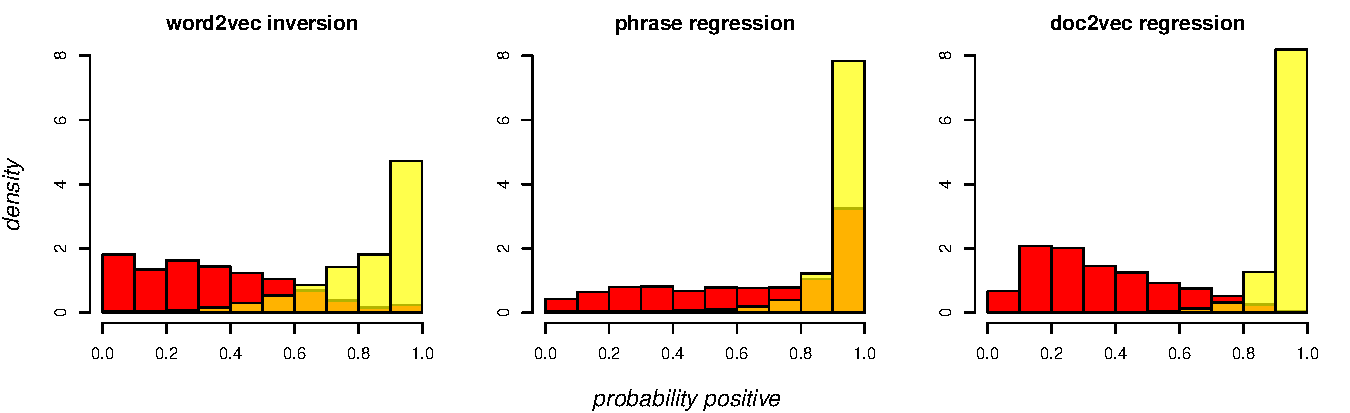
\includegraphics[width=\textwidth]{../graphs/coarseprob}

\vskip .5cm
\begin{center}
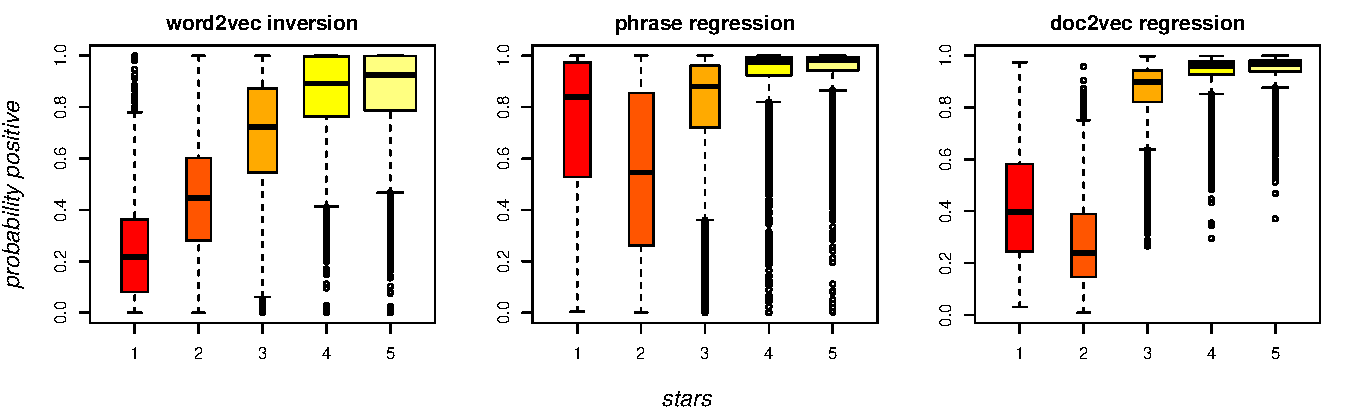
\includegraphics[width=.98\textwidth]{../graphs/coarseprob_bystar}
\end{center}
\vskip -.25cm
\caption{\label{pic:coarseprob} Out-of-Sample fitted probabilities of a review having greater than 2 stars. In the top histograms, red (dark) are the probabilities for true negative reviews and yellow (light) are for true positives.}
\end{figure*}
 


\begin{figure*}
\begin{center}
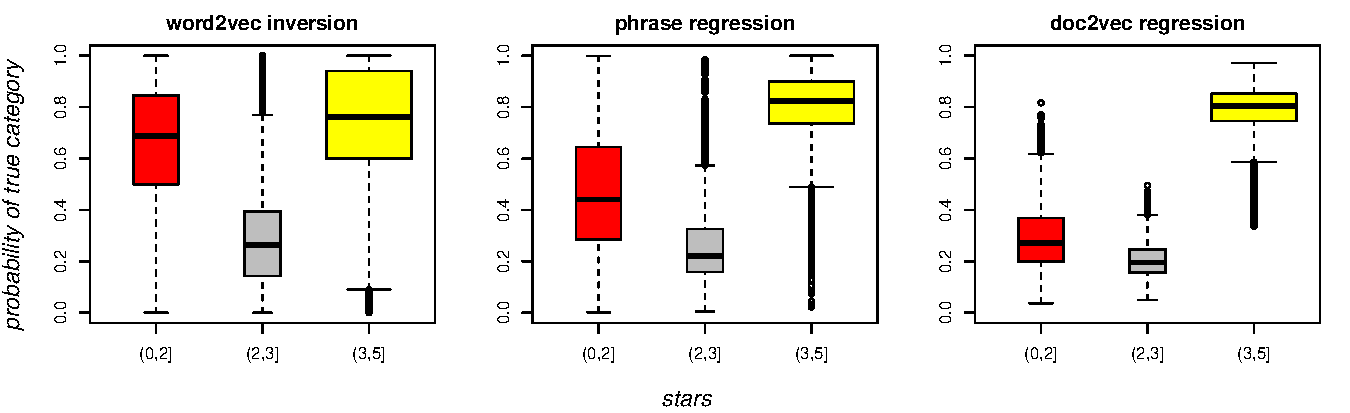
\includegraphics[width=.98\textwidth]{../graphs/nnpprob}

\vskip .25cm

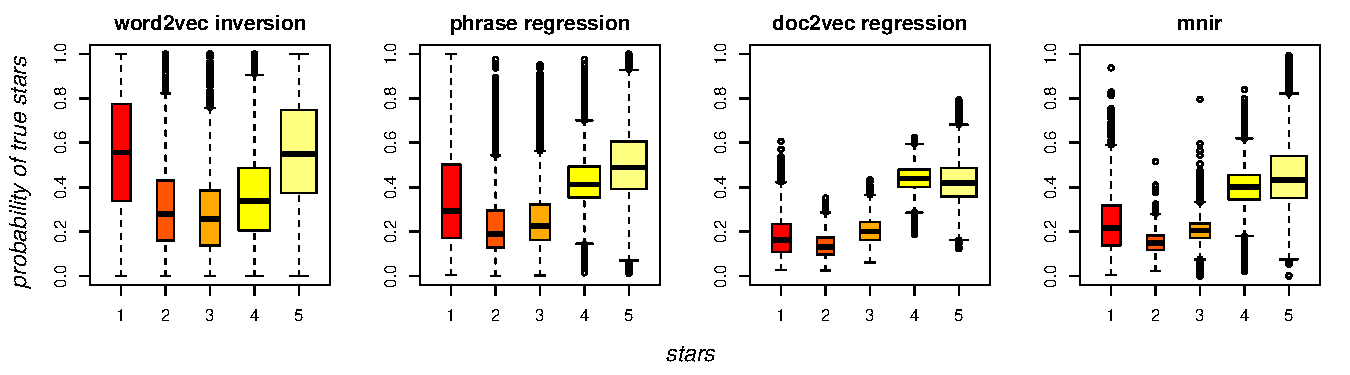
\includegraphics[width=.98\textwidth]{../graphs/fineprob}
\end{center}
\vskip -.25cm
\caption{\label{pic:fineprob} Out-of-Sample fitted probabilities for  observed truth.  In the top plot, we are predicting Negative ($\leq 2$), Neutral ($3$), or Positive ($\geq 4$).  In the bottom, we are predicting each of the separate 5 star ratings.}
\end{figure*}
 

\bibliographystyle{acl}
\bibliography{deepir}


\end{document}
